\chapter{Variational methods in Image Processing}
\label{chapter:variational-methods-in-image-processing}

\section{Inverse problems}
%In the music world, nothing is as complex as an orchestra score. You have plenty of instruments following different tones, dynamics, intensities, rhythms and so on. But no matter the complexity, given the orchestra score a software can reproduce with perfection the piece of music. It is a totally  different story if you ask it to create the orchestra score from an audio file. Reading the score is a forward problem, and creating the score is an inverse problem.

An archaeological museum decided to digitize all its collection and make them available for digital visits over the internet. The chosen method of digitization consists into take a set of pictures, in different camera positions, for each object and then to use a stereo algorithm to assemble all the pieces and create a 3D model of the object. The stereo problem is an \emph{inverse problem}.

Inverse problems are characterized by a degree of \emph{uncertainty} or \emph{lack of information}. The 2D pictures in the problem above miss depth information, that should be \emph{inferred} by the stereo algorithm. On the other hand, if the shape geometry was known precisely, i.e., the values of mean curvature were known for every infinitesimal point of the shape, then constructing a digital 3D representation would be a \emph{direct problem}. In few words, direct problems deals with predictions and inverse problems deals with inference.

Inverse problems are ubiquitous in science. We can find examples in natural language processing, signal processing, geophysics, astronomy and machine learning, for example. In fact, a great part of real world applications consists into infer parameters of some model, i.e., an inverse problem. In~\cref{ch1:tab:inverse-problems-list} we list some examples of inverse problems and its corresponding direct problem version.

\begin{table}
\footnotesize
\begin{tabular}{|m{6cm}|m{5cm}|m{5cm}|}
\hline
Direct problem & Inverse problem & Lack of information / Uncertainty \\
\hline
Compute the projection $P(v)$ of vector $v \in R^3$ in $R^2$ & Infer the vector $v$ from its projection $P(v)$ & Lacking information in one dimension\\
\hline
Given a random variable $X$ following a Gaussian distribution with parameters $(\mu=0,\sigma=1)$, compute the probability $P(X=0.42)$ & Given a set of observations $\Gamma$, infer the parameters that best describes $\Gamma$ as realizations of a Gaussian distribution with parameters $(\mu,\sigma)$ &  Mean and standard deviation missing\\
\hline
Given an image $I$, add some random noise to $I$ to produce image $I'$ & Given the corrupted image $I'$, infer the original image $I$ & We don't know which pixels are corrupted or not \\
\hline
Given an image $I$, compute the image $I'$ resulting from the removal of a patch $P \subset  I$ & Given image $I'$, reconstruct image $I$ & Patch is missing\\
\hline
Given a partition $\mathcal{I}$ of some image $I$, assemble the pieces to create image $I$ & Given image $I$, find the partition $\mathcal{I}$ & Lack information on the partition\\
\hline
\end{tabular}
\caption{Examples of inverse problems and its direct versions. Inverse problems are characterized by uncertainty and parameter inference. }
\label{ch1:tab:inverse-problems-list}
\end{table}

In mathematics, uncertainty is very often translated in to ill-posed problems. An ill-posed problem is a problem that is not well-posed. A well-posed problem, on the other hand, must respect the two conditions below.

\begin{enumerate}
\item{A solution exists and it is unique;}
\item{The solution changes continuously with its parameters}
\end{enumerate}



In~\cref{ch1:tab:inverse-problems-list} all the inverse problems are ill-posed. In order to solve ill-posed problems one should include additional information, i.e., create assumptions over the properties of searched solution. For example, one may assume that vector $v$ is at some distant $d$ of $P(v)$ for the projection problem. The solution set, in this case, is restricted to two. The process of including additional information in ill-posed problems is called \emph{regularization} and its goal is to transform ill-posed problems in well-posed ones.

\section{Image model}
As remarked in the previous section, inverse problems involve some level of uncertainty about the solution. In order to solve an ill-posed problem we need to regularize it by including additional information, or assumptions. To simplify notation, we limit our discussion to grayscale images, the concepts being extendable to multichannel images. It is convenient to have in mind two different representations of an image. \\

\begin{center}
\begin{tabular}{rl}
	Continuous: & $f_I: \Omega \subset \mathbb{R}^2 \rightarrow \mathbb{U}$ \\
	Discrete: & $I \in \mathbb{F}^{m \times n}$,
\end{tabular}
\end{center}

where $\mathbb{F}$ is a finite set, e.g., $\{ i \; | \; i \in \mathbb{N}, i \leq 255 \}$. The discrete representation is interpreted as a sampling of $m \times n$ elements (pixels) of the continuous function $f_I$. 

\section{Image denoising}

\subsection{Bayesian rationale}

Let's consider the denoising problem in the discrete scenario. We are given a corrupted image $\vec{\widetilde{I}} \in \mathbb{U}^{m \times n}$ and we wish to recover the original image $\vec{I}$. As our first assumption, we assume that the corrupted image $\widetilde{I}$ is produced by a matrix $\vec{N} \in \mathbb{U}^{m \times n}$ of random variables $\vec{N}_{i,j}$ following a normal Gaussian distribution, i.e, 

\begin{align}
	\vec{\widetilde{I}} &= \vec{I} + \vec{N},
	\label{ch1:eq:gaussian-noise-model}
\end{align} 

where $Pr\big( \vec{N}_{i,j} = n \big) = \frac{1}{\sqrt{2\pi}}exp( \frac{n^2}{2} )$. We are going to estimate the original image $\vec{I}$ as the image $\vec{I}^{\star}$ that is more likely to occur following~\cref{ch1:eq:gaussian-noise-model}, i.e., 

\begin{align}
	\vec{I}^{\star} & = \argmax _{\vec{C}}{Pr(\vec{C} \; | \;\vec{\widetilde{I}})} = \argmax _{\vec{C}} \frac{Pr(\vec{\widetilde{I}} \; | \; \vec{C})Pr(\vec{C})}{Pr(\vec{\widetilde{I}})},
	\label{ch1:eq:probability-maximization}
\end{align}

where the last expression was derived by applying Bayes' theorem. From~\cref{ch1:eq:gaussian-noise-model} we derive the probability of having the corrupted image $\vec{\widetilde{I}}$ given the original image $\vec{I}$, i.e.,

\begin{align}
	Pr(\vec{\widetilde{I}} \; | \; \vec{C}) &= Pr( \vec{N} = \vec{\widetilde{I}} - \vec{C} ) = \frac{1}{\sqrt{2\pi}}exp\Big(- \frac{ \norm{\vec{\widetilde{I}} - \vec{C} }^2}{2} \Big).
	\label{ch1:eq:probability-corrupted-image-given-original}
\end{align}

Next, we make our second assumption. We are going to favor candidate images that respect some desirable property for the problem to be solved. A popular one for denoising is to assume that the image is piecewise smooth, i.e., its made of closed regions of smooth variations in the color intensity in its interior but with strong discontinuities in their boundaries. There are several ways to model this property. For the moment, let's simply assume that $Pr(\vec{C}) = exp\big(-\rho(\vec{C})\big)$. The denominator term in~\cref{ch1:eq:probability-maximization} is computed as

\begin{align*}
	Pr(\widetilde{\vec{I}}) &= \sum_{\vec{J} \in \mathbb{F}^{m \times n}}{Pr(\vec{\widetilde{I}}\;|\; \vec{J})Pr(\vec{J})} = \frac{1}{\sqrt{2 \pi}}\sum_{\vec{J} \in \mathbb{F}^{m \times n}}{exp\bigg(-\frac{1}{2}\norm{\widetilde{\vec{I}}-\vec{J}}^2 - \rho(\vec{J})}\bigg).
\end{align*}

and~\cref{ch1:eq:probability-maximization} is expanded as

\begin{align}
	\vec{I}^{\star} & = \argmax _{\vec{C}} \frac{1}{\sqrt{2\pi}} \frac{exp\Big(- \frac{1}{2}\norm{\vec{\widetilde{I}} - \vec{C}}^2 - \rho(\vec{C}) \Big) }{ \sum_{\vec{J} \in \mathbb{F}^{m \times n}}{exp\bigg(-\frac{1}{2}\norm{\widetilde{\vec{I}}-\vec{J}}^2 - \rho(\vec{J})}\bigg) }
	\label{ch1:eq:probability-maximization-expanded}
\end{align}

Finnaly, solving~\cref{ch1:eq:probability-maximization-expanded} is equivalent to solve

\begin{align}
	\vec{I}^{\star} &= \argmin _{\vec{C}} \frac{1}{2}\norm{\vec{\widetilde{I}} + \vec{C}}^2 + \rho(\vec{C}).
	\label{ch1:eq:minimization-form}
\end{align}

The first term appears so often in image processing that it has a special name: \emph{data fidelity}. In the denoising problem, the data fidelity term appeared as a consequence of the Gaussian noise model assumption. The second term is also a regularization term, in this case modeling our assumption that the original image is piecewise smooth. We can follow this reasoning for each new assumption we made. The consequence being an additional term in~\cref{ch1:eq:minimization-form}.

\subsubsection{ Euler-Lagrange equation }

A popular way to optimize~\cref{ch1:eq:minimization-form} is to shift it to a continuous setting, analytically derive optimization properties and then use this properties to solve the problem in a discrete setting. The continuous reformulation of~\cref{ch1:eq:minimization-form} consists in to optimize the energy functional below

\begin{align}
	f_{I^{\star}} &= \argmin_{f} F(f) = \frac{1}{2} \int_{\Omega}{ \norm{ f_{\widetilde{I}} - f}^2dx} + R(f)
	\label{ch1:eq:variational-formulation}
\end{align}

\subsection{Tikhonov regularization}

The Tikhonov regularization sets term $R(f)$ as

\begin{align*}
	R(f) &= \int_{\Omega}{ \norm{ \nabla f }^2 dx }.
\end{align*}

The Tikhonov term favors images with smooth variations in color, but the smooth is not restricted to the interior of regions. Thus, Tikhonov tends to obfuscate the discontinuities set and the image appears to be blurred (see~\cref{ch1:fig:denoising-results}). Nonetheless, Tikhonov term is attractive due to its optimization properties.

Assume that function $g$ minimizes functional $F$, i.e.,

\begin{align*}
	g &= \argmin_{f}{F(f)}.
\end{align*}

Further, assume that there exists a function $w$ such that $w=0 \in \partial \Omega$. Define the function $h$ as

\begin{align*}
	h(\epsilon) &= F(g+\epsilon w).
\end{align*}

Therefore, $h$ achieves an extreme value for $\epsilon=0$. Thus,

\begin{align*}
	0 = \frac{dh}{\partial \epsilon}_{| \epsilon=0} &= \frac{d}{\partial \epsilon}_{| \epsilon=0} \frac{1}{2} \int_{\Omega}{ \norm{f_{\widetilde{I}} - g - \epsilon w}^2 + \norm{ \nabla (g + \epsilon w) }^2} \\
	&= _{| \epsilon = 0} \frac{1}{2} \int_{\Omega}{ 2\norm{f_{\widetilde{I}} - g - \epsilon w}\frac{(f_{\widetilde{I}} - g - \epsilon w) }{\norm{f_{\widetilde{I}} - g - \epsilon w}}w + 2\norm{ \nabla (g + \epsilon w) }\frac{(\nabla g + \epsilon w)}{\norm{ \nabla (g + \epsilon w) }}\nabla w} \\
	&= \int_{\Omega}{ (f_{\widetilde{I}} - g)w + (\nabla g)\nabla w}. 	
\end{align*}

Applying integration by parts and using the fact that $w(x)=0,\; \forall x \in \partial Omega$.

\begin{align*}
		0 &= \int_{\Omega} ( f_{\widetilde{I}} - g - \Delta g )w
\end{align*}

Since $w$ could be any function, we can write

\begin{align}
	f_{\widetilde{I}} - g - \Delta g &= 0
	\label{ch1:eq:variational-necessary-condition}
\end{align}

%Therefore, if $g$ is a minimum of~\cref{ch1:eq:variational-formulation}, then it respects ~\cref{ch1:eq:variational-condition}. ~\cref{ch1:eq:variational-formulation} can be proven to be convex. Hence, given an initial solution $f$, one can define a finite differences scheme for $\nabla f$ and apply a descent method (gradient descent) which evolves $f_0$ accordingly with the vector  The next step would be to apply some finite difference scheme to estimate $\nabla g$

Therefore, if $g$ is a minimum of~\cref{ch1:eq:variational-formulation}, then it respects ~\cref{ch1:eq:variational-necessary-condition}. ~\cref{ch1:eq:variational-formulation} can be proven to be convex. Hence, given an initial solution $f$, one can execute a descent method (gradient descent, for example) to find the minimum of~\cref{ch1:eq:variational-formulation}. In practice, ~\cref{ch1:eq:variational-formulation} is discretized using the samplings $I,\widetilde{I}$ of $f_I,f_{\widetilde{I}}$ and a finite differences scheme is defined to estimate the Laplacian $\Delta$.

\subsection{Total variation regularization}
An alternative to Tikhonov regularization is to use the so called total variation of the image function. The problem to be minimized is then defined as

\begin{align}
	f_{I^{\star}} &= \argmin_{f} \frac{1}{2} \int_{\Omega}{ \norm{ f_{\widetilde{I}} - f}^2dx} + \int_{\Omega}{ \norm{\nabla f} dx}.
\end{align}

The $L1$ norm favors smooth interiors and it is less aggressive in the boundaries. Moreover, there are efficient algorithms to solve it~\cite{rudin92,chambolle04,beck09}.

\begin{figure}
\subfloat[Original]{
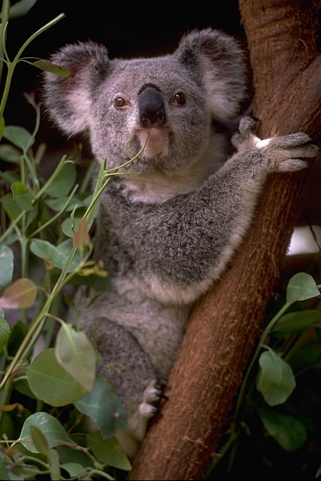
\includegraphics[scale=0.38]{figures/chapter2/denoising/coala-original.png}
}%
\subfloat[Noisy]{
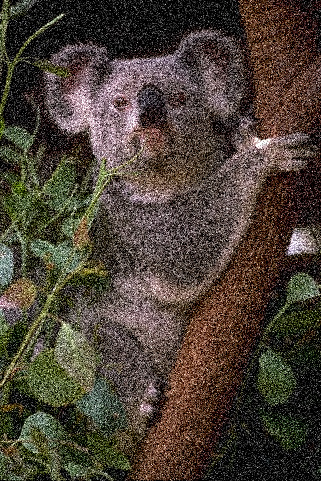
\includegraphics[scale=0.38]{figures/chapter2/denoising/coala-noise.png}
}%
\subfloat[Tikhonov]{
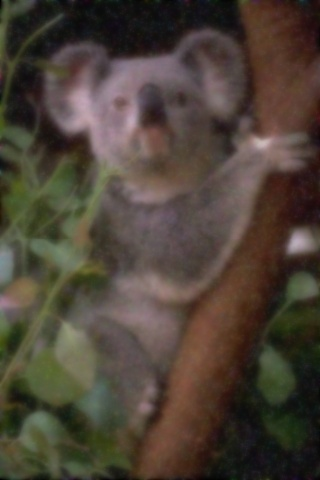
\includegraphics[scale=0.38]{figures/chapter2/denoising/coala-tikhonov.png}
}%
\subfloat[Total Variation]{
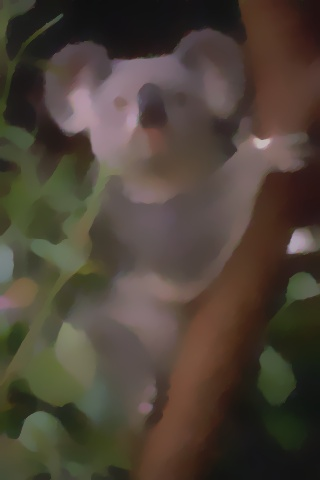
\includegraphics[scale=0.38]{figures/chapter2/denoising/coala-chambolle.png}
}%
\caption{Denoising algorithms results for the Tikhonov and Total variation regulararization terms.}
\label{ch1:fig:denoising-results}
\end{figure}

\section{Image segmentation}
\subsection{Length regularization terms}
\subsection{Mumford-Sha}
\subsection{Chan-Vese}
\subsection{Active contours}

\section{Image inpainting}
\subsection{Level sets completion}



%There is an equivalence between Gibbs distributions and MRF.
%
%Maximum a posteriori is also called penalized maximum likelihood
%
%Consider the problem to find $x$ such that $Ax=b$. If the problem has none or several solutions, the problem is said do be ill-posed. The standard method to solve it is by least-squares plus a penalty term. $|Ax-b|^2 + \lambda P$. The term $P$ models a preference for solutions with some desirable property, e.g., $P=|x|^2$ will favor solutions with lower norm.
%
%Tikhonov regularization is a type of L2 regularization. It is known to improve the problem conditioning and to enable direct solutions (wikipedia article).